\chapter{Koordinatensysteme}\label{ch:kos}
Mit Hilfe von Koordinatensystemen kann der Anschauungsraum geeignet beschrieben werden. Im Kapitel \ref{ch:mathGrundl} wurde im Rahmen des Einf\"uhrungsbeispiels bereits eine Darstellung f\"ur Koordinatensysteme entworfen. F\"ur die Entwicklung eines Koordinatensystems werden die Koordinatenachsen ben\"otigt, welche durch geeignete Geraden beschrieben werden. Die Richtung der Geraden wird durch die \textit{Einheitsvektoren} definiert. Die Koordinatenachsen schneiden sich im \textit{Koordinatenursprung}. Durch die Festlegung dieser Elemente kann die Position eines Punktes im Raum als Vektor beschrieben werden. \hfill \newline
Zur Beschreibung des Anschauungsraums werden genau drei Koordinatenachsen mit drei Einheitsvektoren und einem Ursprungspunkt ben\"otigt. Die drei Einheitsvektoren m\"ussen so gew\"ahlt werden, dass sie einen Vektorraum entsprechend Definition \ref{def:mathGrundl_vektorraeume_vektorraum} aufspannen, sie bilden also eine Basis nach Definition \ref{def:mathGrundl_vektorraeume_basis}. Die Position eines Raumpunktes kann dann durch einen Ortsvektor beschrieben werden, welcher ein Element eben dieses Vektorraumes ist. Dieser Ortsvektor l\"asst sich als eine nach Definition \ref{def:mathGrundl_vektorraeume_linearKombi} gegebene Linearkombination  der Basisvektoren darstellen. Seine Darstellung ist abh\"angig von der konkreten Basis. \hfill \newline
Zun\"achst soll ein besonderer Typ von Koordinatensystemen beschrieben werden - die Rechtssysteme. Diese sind ein grundlegendes Mittel, um die Bewegung von K\"orpern zu beschreiben. 
Da die Festlegung einer Basis f\"ur einen Vektorraum nicht eindeutig ist, kann die Darstellung von einem Koordinatensystem nicht eindeutig sein. Die Umrechnung verschiedener Varianten geschieht mit Hilfe von Transformationen. Die Transformation von einem k\"orperfesten in ein inertiales Koordinatensystem kann durch die \"Uberlagerung einer Translation und einer Rotation abgebildet werden. Auf die Rotation wird im Abschnitt \ref{ssec:kos_transfHomog_rots} im Detail eingegangen. \hfill \newline
Die Elemente von Rechtssystemen werden als Elemente des $\set{R}^{3}$ aufgefasst und \"ublicherweise mit Hilfe von genau drei Komponenten $\left(x, y, z \right)^{T}$ notiert. Diese Darstellung kann durch eine zus\"atzliche Komponente zu einem 4-Tupel erweitert werden. Die so erhaltenen \textit{homogenen Koordinaten} werden im Abschnitt \ref{ssec:kos_transfHomog_homKoord} eingef\"uhrt und es wird auf deren besondere Eigenschaften eingegangen. Insbesondere kann die Transformation von Koordinatensystemen, welche im Abschnitt \ref{ssec:kos_transfHomog_transf} erl\"autert wird, unter Verwendung homogener Koordinaten kompakt durch lineare Abbildungen dargestellt werden. \hfill \newline
Bei der Beschreibung eines Mehrk\"orpersystems gibt es vielf\"altige Ans\"atze um die Lage einzelner Elemente zu parametrieren. Ein m\"oglicher Ansatz ist die Vorgabe nat\"urlicher Koordinaten, welche im Abschnitt \ref{sec:kos_natKoord} beschrieben werden. Im letzten Teil des Kapitels werden wichtige Begriffe erkl\"art und es wird auf weitere Konzepte zur Modellbildung verwiesen.
 
 \section{Kartesische normierte Rechtssysteme}\label{sec:kos_rechtssys}
  Gegeben sei ein euklidisches Koordinatensystem \footnote{mit dem Begriff euklidisches Koordinatensytem wird ein Koordinatenraum $\set{R}^{3}$ mit Skalarprodukt nach \eqnref{gl:mathGrundl_punkteVektoren_skalarProd} bezeichnet} $\KOS{I}\in \R^{3}$ mit den Basisvektoren $\vect{e}_1,\vect{e}_2,\vect{e}_3$. F\"ur die Basisvektoren gelte: \begin{align}
\skalar{\vect{e}_i}{\vect{e}_j}&=
\begin{cases}
1, \text{ f\"ur } i=j \\
0, \text{ f\"ur } i\neq j \end{cases} \label{gl:kos_orthosys}
\end{align}
Die Basisvektoren von $\KOS{I}$ stehen also paarweise senkrecht aufeinander und bilden somit ein \textit{orthogonales} Koordinatensystem. Ein orthogonales euklidisches Koordinatensystem wird als \textit{Kartesisches Koordinatensystem} bezeichnet. Weiterhin ist die L\"ange jedes Basisvektors gleich eins. Die Basis wird daher als \textit{normiert} bezeichnet und das aufgespannte Koordinatensystem als orthonormiertes System bezeichnet.\hfill \newline
Gilt au\ss{}erdem \begin{align}
\vect{e}_1 \times \vect{e}_2 &= \vect{e}_3, \label{gl:kos_rechtssys}
\end{align}
so bezeichnet man $\KOS{I}$ als ein rechtsh\"andiges Koordinatensystem oder auch Rechtssystem. Eine anschauliche Interpretation von \eqnref{gl:kos_rechtssys} ist, dass jeder Einheitsvektor aus seinem Vorg\"anger auf k\"urzestem Wege durch Drehung im mathematisch positiven Drehsinn  hervorgeht. Der Vektor $\vect{e}_{1}$ ist in diesem Sinne gleichzeitig der Nachfolger vom Einheitsvektor $\vect{e}_{3}$ und der Vorg\"anger von $\vect{e}_{2}$, welcher wiederum der Vorg\"anger von $\vect{e}_{3}$ ist. \hfill \newline
Im Folgenden wird, wenn nicht explizit anderweitig angegeben, davon ausgegangen, dass die Basisvektoren eines Koordinatensystems \eqnref{gl:kos_orthosys} und \eqnref{gl:kos_rechtssys} erf\"ullen.  
\begin{exmp}[Kartesischen Rechtssystem]\label{exmp:sec:kos_rechtssys_stdBasis} Mit Hilfe der in Bemerkung \ref{rem:mathGrundl_vektorraeume_kanBasis} angegeben Bildungsvorschrift l\"asst sich auf einfache Weise eine Basis f\"ur ein kartesisches Rechtssystem angeben: \begin{align*}
\vect{e}_{1}&=\begin{pmatrix}
1 \\ 0 \\0
\end{pmatrix} &\vect{e}_{2}&=\begin{pmatrix}
0 \\ 1 \\0
\end{pmatrix} &\vect{e}_{3}&=\begin{pmatrix}
0 \\ 0 \\1
\end{pmatrix}
\end{align*}
\end{exmp}
  
  \section{Koordinatentransformation in homogenen Koordinaten}\label{sec:kos_transfHomog}
 % \subsection{hilfreiche Literatur}
 % \cite[S.10]{Pfeiffer2014}
  \subsection{Rotationen und deren Darstellung mittels Matrizen}\label{ssec:kos_transfHomog_rots}
  \"Andert ein K\"orper seine Orientierung im Raum, so bewegen sich alle Punkte des K\"orpers um eine Drehachse und man bezeichnet diese Bewegung als \textit{Rotation}. Ist die Lage dieser Achse konstant, so bezeichnet man dies als Rotation um eine feste Achse. Verl\"auft die Drehachse durch einen raumfesten Punkt, so handelt es sich um eine Kreiselbewegung. In jedem Fall kann die Drehbewegung durch eine zeitlich ver\"anderliche oder konstante Rotationsmatrix ausgedr\"uckt werden. Zur Formulierung der Rotationsmatrix seien ein k\"orperfestes Koordinatensystem $\KOS{K}$ und ein inertiales Koordinatensystem $\KOS{I}$ gegeben. Die Koordinatensysteme $\KOS{I}$ und $\KOS{K}$ haben weiterhin den gleichen Ursprung. Das System $\KOS{K}$ ist demnach durch Drehung um eine Achse $l$, welche durch den Ursprung verl\"auft, hervorgegangen. Die Orientierung dieser Drehachse sei durch einen Vektor $\vect{l}$ mit Einheitsl\"ange beschrieben. Die Achsen von $\KOS{K}$ relativ zu $\KOS{I}$ seien gegeben durch die Einheitsvektoren $\tensor*[_I]{\vect{u}}{}, \tensor*[_I]{\vect{w}}{}, \tensor*[_I]{\vect{v}}{} \in \R^{3}$. Diese drei Spaltenvektoren werden horizontal zu einer Matrix \begin{align}
  \matr{R}&=\begin{pmatrix}
  \tensor*[_I]{\vect{u}}{}& \tensor*[_I]{\vect{w}}{}& \tensor*[_I]{\vect{v}}{}
  \end{pmatrix} = \begin{pmatrix}
  \tensor*[_I]{u}{_x}& \tensor*[_I]{w}{_x}& \tensor*[_I]{v}{_x} \\ 
  \tensor*[_I]{u}{_y}& \tensor*[_I]{w}{_y}& \tensor*[_I]{v}{_y} \\ 
  \tensor*[_I]{u}{_z}& \tensor*[_I]{w}{_z}& \tensor*[_I]{v}{_z}
  \end{pmatrix} \label{gl:kos_transfHomog_rots_rotMatrDef}
  \end{align}
  zusammengefasst. Die Matrix $\matr{R}$ wird als Rotationsmatrix oder Drehmatrix bezeichnet. Sie gibt die relative Verdrehung von $\KOS{K}$ zu $\KOS{I}$ an. Die Spaltenvektoren, welche zur Matrix $\matr{R}$ zusammengefasst werden, sind im Folgenden, wenn nicht explizit anderweitig angegeben, in der Basis des Inertialsystems angegeben. \hfill \newline 
  Die Rotationsmatrix $\matr{R}$ kann auch durch Verwendung einer absoluten Angabe der Einheitsvektoren beider Koordinatensysteme angegeben werden. Bilden die Einheitsvektoren $\tensor*[_I]{\vect{e}}{_1}, \tensor*[_I]{\vect{e}}{_2}, \tensor*[_I]{\vect{e}}{_3} \in \set{R}^{3}$ eine Basis von $\KOS{I}$ und die Vektoren $\tensor*[_K]{\vect{u}}{}, \tensor*[_K]{\vect{w}}{}, \tensor*[_K]{\vect{v}}{}$ die Basis f\"ur $\KOS{K}$, so k\"onnen diese Spaltenvektoren geeignet als Matrizen angeordnet werden und die Rotationsmatrix, welche die Verdrehung von $\KOS{K}$ relativ zu $\KOS{I}$ angibt, wie folgt berechnet werden:
  \begin{align*}
  \matr{B}_{K}= \begin{bmatrix}
  \tensor*[_K]{\vect{u}}{}& \tensor*[_K]{\vect{w}}{}& \tensor*[_K]{\vect{v}}{} \end{bmatrix} &= \begin{bmatrix}
  \tensor*[_K]{u}{_x}& \tensor*[_K]{w}{_x}& \tensor*[_K]{v}{_x} \\ 
  \tensor*[_K]{u}{_y}& \tensor*[_K]{w}{_y}& \tensor*[_K]{v}{_y} \\ 
  \tensor*[_K]{u}{_z}& \tensor*[_K]{w}{_z}& \tensor*[_K]{v}{_z}
\end{bmatrix}\\
  \matr{B}_{I}= \begin{bmatrix}
  \tensor*[_I]{\vect{e}}{_1}& \tensor*[_I]{\vect{e}}{_2}& \tensor*[_I]{\vect{e}}{_3} \end{bmatrix} &= \begin{bmatrix}
  \tensor*[_I]{e}{_{1,x}} & \tensor*[_I]{e}{_{2,x}} & \tensor*[_I]{e}{_{3,x}} \\ 
  \tensor*[_I]{e}{_{1,y}} & \tensor*[_I]{e}{_{2,y}} & \tensor*[_I]{e}{_{3,y}} \\ 
  \tensor*[_I]{e}{_{1,z}} & \tensor*[_I]{e}{_{2,z}} & \tensor*[_I]{e}{_{3,z}}
\end{bmatrix} 
\end{align*}
\begin{align}
  \tensor*[^K_I]{\matr{R}}{}&= \inv{\matr{B}_{I}} \matr{B}_{K} \label{gl:transfHomog_rots_rotMatrAllg}
  \end{align}
  Handelt es sich bei der Basis von $\KOS{I}$ um eine Standardbasis, wie sie im Beispiel \ref{exmp:sec:kos_rechtssys_stdBasis} angegeben ist, so vereinfacht sich  \eqnref{gl:transfHomog_rots_rotMatrAllg} zu \begin{align}
  \matr{R}&= \matr{B}_{K}.
  \end{align}
    \subsubsection{Eigenschaften von Rotationsmatrizen}\label{sssec:kos_transfHomog_rots_eigensch}
    Entsprechend \eqnref{gl:kos_transfHomog_rots_rotMatrDef} seien die Vektoren $\vect{u}, \vect{w}, \vect{v} \in \R^{3}$ die Spalten der Rotationsmatrix $\matr{R}\in \R^{3\times 3}$. Da diese ein Koordinatensystem aufspannen sollen, haben sie die in \eqnref{gl:kos_orthosys} und \eqnref{gl:kos_rechtssys} definierten Eigenschaften. Aus \eqnref{gl:kos_orthosys} folgt f\"ur die Matrix $\matr{R}$ \begin{align}
    \matr{R}\transp{\matr{R}} &= \begin{pmatrix}
    \vect{u} & \vect{w}& \vect{v} 
\end{pmatrix} \begin{pmatrix}
\vect{u}\\ \vect{w}\\ \vect{v}  
\end{pmatrix} =      \transp{\matr{R}}\matr{R} = \matr{I} \label{gl:rotMatrTransp}
\intertext{was umgeformt werden kann zu}
\transp{\matr{R}}&= \inv{\matr{R}}. \label{gl:kos_transfHomog_rots_eigensch_inv}
    \intertext{Mit Hilfe der Regeln der linearen Algebra \cite[S. 100]{Papula2014} und \eqnref{gl:kos_orthosys} folgt aus \eqnref{gl:rotMatrTransp}}
    \det{\matr{R}} &= \skalar{\vect{u}}{\vect{w}\times \vect{v}}= \skalar{\vect{u}}{\vect{u}} =  1. \label{gl:rotMatrDet}
\end{align} Die Menge der orthogonalen $3 \times 3$ Matrizen mit der Determinante eins wird als $\set{SO}\of{3}$ bezeichnet \cite{Murray1994}. Allgemein wird definiert: \begin{align}
\set{SO}\of{n} = \left \lbrace \matr{R}\in \R^{n\times n}: \matr{R}\transp{\matr{R}}=\matr{I}, \det{\matr{R}}=+1 \right \rbrace. \label{gl:mengeSoDef}
\end{align} Die Menge $\set{SO}\of{3}\subset \R^{3\times 3}$ bildet mit der Abbildungsvorschrift \textit{Matrixmultiplikation} eine Gruppe entsprechend den im Abschnitt \ref{sec:mathGrundl_gruppen} geforderten Regeln. Sie wird als \textit{spezielle orthogonale Gruppe} bezeichnet. Die Elemente dieser Gruppe erhalten die Rechtsh\"andigkeit von Koordinatensystemen. Die geforderten Eigenschaften eine Gruppe werden wie folgt erf\"ullt:
\begin{itemize}
\item Die Verkn\"upfung ist abgeschlossen. F\"ur $\matr{R}_1, \matr{R}_2 \in \set{SO}\of{3}$ gilt auch $\matr{R}_1 \matr{R}_2 \in \set{SO}\of{3}$, da \begin{align}
\matr{R}_1 \matr{R}_2 \transp{\of{\matr{R}_1 \matr{R}_2}} &= \matr{R}_1 \matr{R}_2 \transp{\matr{R}_2} \transp{\matr{R}_1} = \matr{R}_1 \transp{\matr{R}_1} = \matr{I} \\ \label{gl:kos_transfHomog_rots_eigensch_abgeschl}
\det\of{\matr{R}_1 \matr{R}_2} &= \det\of{\matr{R}_1} \det\of{\matr{R}_2} = +1
\end{align} gilt.
\item Die Gruppe $\set{SO}\of{3}$ ist assoziativ \begin{align}
\intertext{Aus der Assoziativit\"at der Matrixmultiplikation (Beweis siehe z. B. \cite[s. 93]{Bosch2014}) folgt}
\left( \matr{R}_1 \matr{R}_2\right) \matr{R}_3 &= \matr{R}_1 \left(\matr{R}_2 \matr{R}_3 \right) \label{gl:mengeSoGruppenAssoz}
\end{align}
\item Die Einheitsmatrix ist das neutrale Element \begin{align}
\matr{I} \matr{R} = \matr{R} \matr{I} = \matr{R} \quad \forall { } \matr{R} \in \set{SO}\of{3} \label{gl:kos_transfHomog_rots_eigensch_neutrElem}
\intertext{mit} 
\matr{I}&=\begin{pmatrix}
1 & 0 & 0\\ 0 & 1 & 0 \\ 0 & 0 & 1
\end{pmatrix} \nonumber
\end{align}
\item Aus \eqnref{gl:rotMatrTransp} folgt, dass $\transp{\matr{R}}\in \set{SO}\of{3}$ das inverse Element von $\matr{R} \in \set{SO}\of{3}$ ist: \begin{align}
\inv{\matr{R}}&= \transp{\matr{R}}.
\end{align}
\end{itemize}
Differenziert man \eqnref{gl:rotMatrTransp} nach der Zeit und beachtet die Zeitabh\"angigkeit der Rotationsmatrizen, so erh\"alt man mit der Produktregel nach \eqnref{gl:mathGrundl_vektorraeume_matr_prodDiff} \begin{align} \label{gl:kos_transfHomog_rots_eigensch_winkelMatr} \begin{split}
\frac{\d \matr{I}}{\d t}&=  \frac{\d {\matr{R}\of{t}\transp{\matr{R}}\of{t}}}{\d t}
 \\
\implies 0&= \dot{\matr{R}}\of{t}\transp{\matr{R}}\of{t} + \matr{R}\of{t}\transp{\dot{\matr{R}}}\of{t} 
 \\
\com{\dot{\matr{R}}\of{t}\transp{\matr{R}}\of{t}}{$:=\matr{\Omega}$} &= - \matr{R}\of{t}\transp{\dot{\matr{R}}}\of{t} 
 \\
\matr{\Omega} &= - \transp{\matr{\Omega}}  \end{split}
\end{align}
Die so definierte Matrix $\matr{\Omega}$ erf\"ullt also offensichtlich \eqnref{gl:SdT_mathGrundl_punkteVektoren_kreuzProdOp_transp} und ist daher schiefsymmetrisch. Die Bedeutung dieser Matrix wird im Abschnitt \ref{sec:mech_starrkoerperbewegung} erl\"autert.
\begin{rem}[Eigenvektor von $\matr{R}$] Die Matrix $\matr{R}$ hat die besondere Eigenschaft, dass ihr Eigenvektor mit dem Eigenwert gleich eins der Drehachse entspricht, um welche die Rotation durchgef\"uhrt wird. 
\end{rem}

\begin{rem} Die Lage eines Starrk\"orpers, welcher sich frei im Raum drehen kann, kann zu jedem Zeitpunkt durch eine eindeutige Rotationsmatrix $\matr{R}\in \set{SO}\of{3}$ beschrieben werden. Die Menge der Rotationsmatrizen $\set{SO}\of{3}$ wird daher als der Konfigurationsraum des Systems bezeichnet. Eine Trajektorie des Systems wird durch die Kurve $\matr{R}\of{t} \in \set{SO}\of{3}$ f\"ur $t\in [0,T]$ abgebildet. Weiterhin dient die Matrix $\matr{R}$ zur Transformation von Punkten von einem k\"orperfesten, um eine beliebige Achse gedrehten, Koordinatensystem in ein Inertialsystem. Insbesondere ist die $3\times 3$ Einheitsmatrix nach \eqnref{gl:kos_transfHomog_rots_eigensch_neutrElem} das neutrale Element der Gruppe der Rotationsmatrizen. Eine Transformation mit dieser Matrix ist damit eine Transformation ohne Drehung. Die allgemeine Transformation von Koordinatensystemen ist im Abschnitt \ref{ssec:kos_transfHomog_transf} genauer dargelegt.
\end{rem}
\subsection{Homogene Koordinaten}\label{ssec:kos_transfHomog_homKoord}
  Die Darstellung von Bewegungen mit Hilfe homogener Koordinaten, wie sie beispielsweise von D. W. Wloka in \cite[S. 72]{Wloka1992} eingef\"uhrt werden, erm\"oglicht eine einheitliche kompakte Darstellung von Translationen und Rotationen eines K\"orpers durch Verwendung einer einzigen Transformationsmatrix. Dazu werden die Vektoren des $\set{R}^{3}$, mit denen der Anschauungsraum beschrieben wird, um eine vierte Komponente erweitert. Dieser \textit{Skalierungsfaktor} wird \"ublicherweise null oder eins gesetzt. Andere Skalierungsfaktoren werden bei der Arbeit mit Computergrafiken verwendet. \hfill \newline
  Transformiert man einen Richtungsvektor, wie er in Abschnitt \ref{ssec:mathGrundl_punkteVektoren_r3} beschrieben wird, so verwendet man die null als Skalierungsfaktor. F\"ur Punkte beziehungsweise Ortsvektoren wird die eins als Skalierungsfaktor benutzt. \hfill \newline
  Gegeben sei ein Vektor $\vect{z}$, welcher zwei beliebige Punkte eines K\"orpers verbindet. Bewegt sich der K\"orper derart, dass dieser Vektor seine Orientierung nicht \"andert, so bezeichnet man diese Bewegung als \textit{Translation}. Die Translation f\"ur den Vektorraum $\set{R}^{3}$ mit dem Vektor $\vect{q}\in \set{R}^{3}$ ist definiert als \begin{align*}
  f&: \vect{r} \longrightarrow \vect{r}+\vect{q} &\vect{r},\vect{q}&\in\set{R}^{3}.
\end{align*} Diese Abbildung ist nicht linear. Es gilt \begin{align*}
f\of{\vect{r}+\vect{y}}&= \vect{r}+\vect{y}+\vect{q},
\end{align*} wodurch \eqnref{gl:mathGrundl_abbildung_linAbb_add} nicht erf\"ullt wird. Die Translation l\"asst sich daher nicht als Matrix darstellen. Man kann aber zeigen, dass die Translation bijektiv ist. Es existiert also eine Umkehrabbildung f\"ur die Translation. K\"onnte man die Translation als Matrix darstellen, so w\"are die Zusammenfassung einer beliebigen Folge von Rotationen und Translationen in einer einzigen Matrix $\matr{A}$ m\"oglich. Jeder K\"orperpunkt, der durch einen Ortsvektor $\vect{r}$ beschrieben werden kann,  lie\ss{}e sich dann nach einer beliebigen Anzahl und Reihenfolge von Verdrehungen und Verschiebungen durch eine einzige Matrix-Vektor-Multiplikation berechnen: $\vect{r}'= \matr{A}\vect{r}$.  Dies wird durch die Einf\"uhrung homogener Koordinaten erreicht.  \hfill \newline 

  \"Ublicherweise notiert man die  Translation eines Vektors $\vect{r}=\transp{\of{x, y, z}}$ mit einem Vektor $\vect{q}=\transp{\of{a, b, c}}$ als\begin{align*}\vect{r}'&= \vect{r}+\vect{q}= \begin{bmatrix}
  x \\ y \\ z
  \end{bmatrix} + \begin{bmatrix}
  a \\ b\\c
  \end{bmatrix} = \begin{bmatrix}
  x+a \\ y+b \\ z+c
  \end{bmatrix}.
  \end{align*} Die Translation entspricht einer additiven Verschiebung des Vektors $\vect{r}$.
  Mit Hilfe einer erweiterten Darstellung kann die Translation als Matrix-Vektor Multiplikation dargestellt werden. Man erweitert dazu den in homogenen Koordinaten gegebenen Vektor $\vect{r}$ um eine $3\times 3$ Einheitsmatrix in homogener Darstellung zu einer $4\times 4$ Matrix und notiert dann \begin{align*}
  \vect{r}' &= \begin{bmatrix}
  \matr{I}^{3\times 3} & \vect{q}\\
  \vect{0} & 1
  \end{bmatrix} \vect{r} \\
  &=\begin{bmatrix}
  1 & 0 & 0& a\\
  0 & 1 & 0& b\\
  0 & 0 & 1& c\\
  0 & 0 & 0& 1\\
  \end{bmatrix} \begin{bmatrix}
  x \\ y \\ z \\1
  \end{bmatrix} = \begin{bmatrix}
  x+a \\ y+b \\ z+c \\ 1
  \end{bmatrix}.
  \end{align*}
  Die Erweiterung zu einer Matrix erfolgt also mit dem nach \eqnref{gl:kos_transfHomog_rots_eigensch_neutrElem} gegebenen neutralen Element der speziellen orthogonalen Gruppe $\set{SO}\of{3}$. \hfill \newline
  Stellt man die Rotation eines K\"orpers mit Hilfe eines Koordinatensystems dar, welches sich mit dem K\"orper mit dreht, so kann die Rotationsmatrix durch die drei Basisvektoren $\vect{u}, \vect{w}, \vect{v}$ dieses Koordinatensystems beschrieben werden. Die Rotationsmatrix $\matr{R}$ schreibt man dann nach \eqnref{gl:kos_transfHomog_rots_rotMatrDef} mit\begin{align*}
  \matr{R}&=  \begin{pmatrix}
  u_x & w_x & v_x \\ u_y & w_y & v_y \\ u_z & w_z & v_z
  \end{pmatrix}.
  \end{align*} Da die drei Spalten dieser Matrix jeweils die Komponenten von Richtungsvektoren enthalten, werden diese bei der Transformation in homogene Koordinaten um den Skalierungsfaktor null erg\"anzt und man notiert \begin{align*}
  \matr{R}&=  \begin{pmatrix}
  u_x & w_x & v_x \\ u_y & w_y & v_y \\ u_z & w_z & v_z \\ 0&0&0
  \end{pmatrix}.
  \end{align*}
  Eine Transformationsmatrix $\matr{T}$, welche die komplette Bewegung eines K\"orpers beinhalten soll, setzt sich aus Rotation $\matr{R}$ und Translation $\vect{q}$ zusammen. Sie wird in homogenen Koordinaten beschrieben mit: \begin{align}
  \matr{T}&= \begin{bmatrix}
  \matr{R} & \vect{q}\\ 
  \vect{0} & 1
  \end{bmatrix} = \begin{pmatrix}
  u_x & w_x & v_x & a\\ u_y & w_y & v_y& b \\ u_z & w_z & v_z& c \\ 0&0&0&1
  \end{pmatrix}. \label{gl:kos_transfHomog_homKoord_transfoKompl}
  \end{align}
  Die Inverse einer solchen Transformationsmatrix berechnet sich unter Beachtung der Orthogonalit\"atseigenschaft von $\matr{R}$ beziehungsweise \eqnref{gl:rotMatrTransp} zu \begin{align}
  \inv{\matr{T}}&= \begin{bmatrix}
  \transp{\matr{R}} & - \transp{\matr{R}}\vect{q}\\ 
  \vect{0} & 1
  \end{bmatrix} \label{gl:kos_transfHomog_homKoord_transfoInv}
  \end{align}
  In Folge dessen, dass die Transformationsmatrix $\matr{T}$ in homogenen Koordinaten invertierbar ist, wird die Transformation von Vektoren bedeutend vereinfacht.

\begin{rem}[Gruppe der homogenen Transformationsmatrizen] Nach dem \textit{Chasles Theorem} kann jede homogene Transformation $\matr{T}$ aus einer Translation und einer Rotation um dieselbe Achse zusammengesetzt werden. Diese Bewegung wird als \textit{Schraubung} bezeichnet. Die Transformationsmatrizen bilden mit der Matrixmultiplikation die \textit{spezielle euklidische Gruppe} $\set{SE}\of{3}$: \begin{align}
\set{SE}\of{3}&= \left \lbrace \begin{bmatrix}
\matr{R} & \vect{q}\\ \vect{0}&1 \end{bmatrix}: \matr{R}\in \set{SO}\of{3}, \vect{q}\in \set{R}^{3} \right \rbrace \label{gl:kos_transfHomog_homKoord_SE3Def}
\end{align}  
\end{rem}

  Soll die Matrix $\matr{T}$ nach der Zeit abgeleitet werden, so muss das Ergebnis dem der enthomogenisierten Form entsprechen. Dabei ist zu beachten, dass ein Geschwindigkeitsvektor offensichtlich nicht die Position eines Punktes beschreibt. Statt dessen wird durch einen Geschwindigkeitsvektor die Richtung und ein Gr\"o\ss{}enma\ss{} f\"ur die Bewegung angegeben. Daher ist der Skalierungsfaktor eines Vektors in homogener Darstellung, auf welchen der Differentialoperator angewandt wurde, gleich null. Die f\"ur die Beschreibung von Bewegungen besonders wichtige Ableitung nach der Zeit lautet damit in homogenen Koordinaten\begin{align}
  \frac{\d}{\d t} \begin{bmatrix}
  \vect{r}\of{t} \\ 0  
\end{bmatrix}  &= \begin{bmatrix}
\frac{\d\vect{q}\of{t}}{\d t} \\ 0
\end{bmatrix}  
  \intertext{f\"ur einen Vektor und}
  \frac{\d\matr{T}\of{t}}{\d t}&= \begin{bmatrix}
  \frac{\d }{\d t}\matr{R}\of{t} & \frac{\d }{\d t}\vect{q}\of{t}\\ 
  \vect{0} & 0
  \end{bmatrix} \label{gl:kos_transfHomog_homKoord_ableitung}
  \intertext{f\"ur eine Matrix.} \nonumber
  \end{align} Die so berechnete Matrix $\dot{\matr{T}}$ ist demnach kein Element der speziellen euklidischen Gruppe, wie sie in \eqnref{gl:kos_transfHomog_homKoord_SE3Def} definiert wurde. 
  \subsection{Transformationen} \label{ssec:kos_transfHomog_transf}
   Gegeben seien ein inertiales Koordinatensystem $\KOS{I}$ und zwei, um eine beliebige Achse in Relation zu $\KOS{I}$ gedrehte, Koordinatensysteme $\KOS{B},\KOS{C}$, welche den gleichen Ursprung wie $\KOS{I}$ besitzen. Weiterhin sei ein Punkt durch einen Ortsvektor $\vect{\tensor*[_B]{r}{}}= \transp{\left( \tensor*[_B]{x}{}, \tensor*[_B]{y}{}, \tensor*[_B]{z}{} \right) }$ im Koordinatensystem $\KOS{B}$ gegeben. Werden die Koordinatenachsen von $\KOS{B}$ durch die Einheitsvektoren $\vect{\tensor*[_I]{e}{_B_1}}, \vect{\tensor*[_I]{e}{_B_2}}, \vect{\tensor*[_I]{e}{_B_3}}$ im Inertialsystem $\KOS{I}$ beschrieben, so kann der Punkt von $\KOS{B}$ nach $\KOS{I}$ durch eine Transformation \"uberf\"uhrt werden: \begin{align*}
  \vect{\tensor*[_I]{r}{}}&= \begin{pmatrix}
 \vect{\tensor*[_I]{e}{_B_1}}& \vect{\tensor*[_I]{e}{_B_2}}& \vect{\tensor*[_I]{e}{_B_3}}
  \end{pmatrix} \begin{pmatrix}
  \tensor*[_B]{x}{}\\ \tensor*[_B]{y}{}\\ \tensor*[_B]{z}{}
  \end{pmatrix} = \tensor*[_I^B]{\matr{R}}{}  \vect{\tensor*[_B]{r}{}}
\end{align*}
  Der linksseitige tiefgestellte Index gibt das System an, in dem ein Vektor definiert wurde. Der rechtsseitige tiefgestellte Index dient der besseren Unterscheidbarkeit von definierten Gr\"o\ss{}en. Im Fall einer Transformationsmatrix $\tensor*[_I^B]{\matr{R}}{}$ gibt der linksseitige hochgestellte Index das Ursprungssystem und der linksseitige tiefgestellte Index das Zielsystem der Transformation an. \hfill \newline  
  Transformationen k\"onnen aneinandergereiht werden. Beschreibt die Transformationsmatrix $\tensor*[_B^C]{\matr{R}}{}$ die Verdrehung von $\KOS{C}$ relativ zu $\KOS{B}$, so erh\"alt man die Transformationsmatrix von $\KOS{C}$ nach $\KOS{I}$ durch eine Kombination der Transformation vom System $\KOS{C}$ in das System $\KOS{B}$ mit der Transformation vom System $\KOS{B}$ in das System $\KOS{I}$. Die Kombination erfolgt dabei durch linksseitige Matrixmultiplikation der jeweiligen Transformationsmatrizen in der angegebenen Reihenfolge. \begin{align*}
  \tensor*[_I^C]{\matr{R}}{}&= \tensor*[_I^B]{\matr{R}}{} \tensor*[_B^C]{\matr{R}}{}
  \end{align*}
   Da entsprechend \eqnref{gl:kos_transfHomog_rots_eigensch_abgeschl} die Menge der Rotationsmatrizen abgeschlossen ist, ist die durch Aneinanderreihung von Drehungen gewonnen Matrix $\tensor*[_I^C]{\matr{R}}{}$ ebenfalls eine Rotationsmatrix. \hfill \newline

\begin{figure}[htb]
\begin{center}
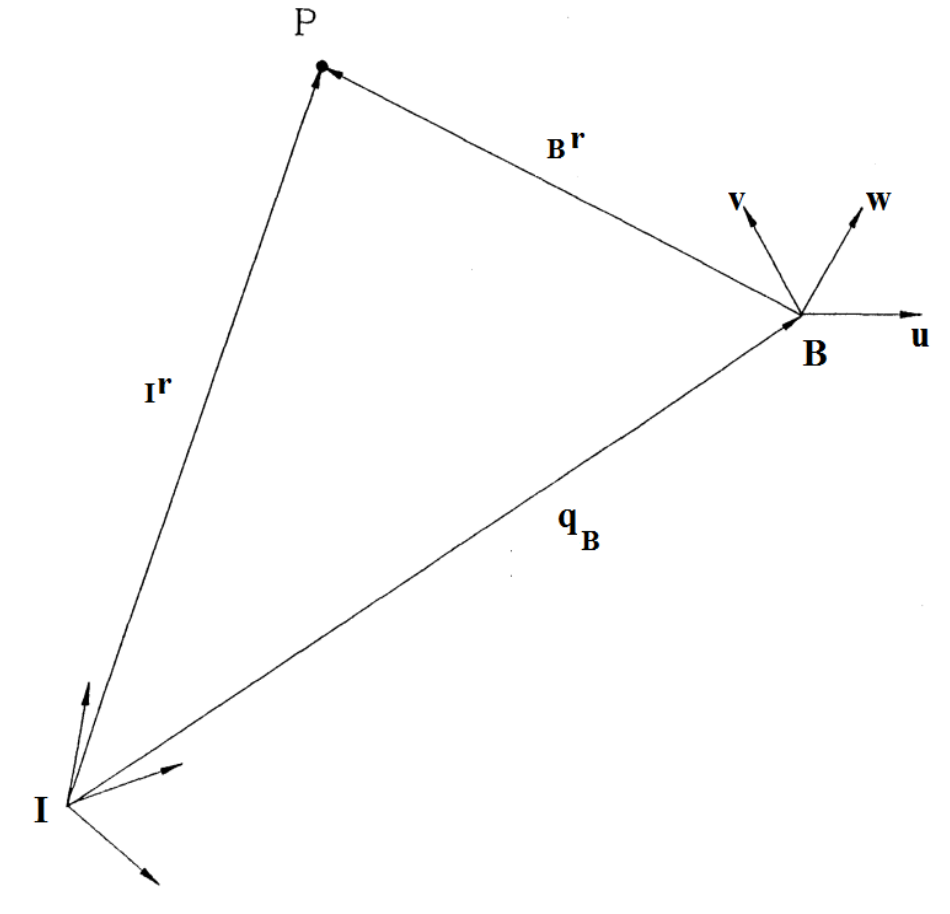
\includegraphics[width=0.5\textwidth]{abbildungen/04_kosTransfo.png}
\caption{Darstellung eines Vektors in verschiedenen Koordinatensystemen}
\label{fig:kos_transfHomog_transf_punktTransfo}
\end{center}
\end{figure}

Sind die Koordinatensysteme $\KOS{B}$ und $\KOS{C}$ zum Inertialsystem nicht nur verdreht, sondern auch um Vektoren $\vect{q}_B, \vect{q}_C$ verschoben, so wird zur Transformation von Vektoren die Transformationsmatrix $\matr{T}$ nach \eqnref{gl:kos_transfHomog_homKoord_transfoKompl} ben\"otigt. F\"ur zwei Systeme $\KOS{I}$ und $\KOS{B}$ ist diese Situation in \figureref{fig:kos_transfHomog_transf_punktTransfo} dargestellt. Ein im System $\KOS{B}$ gegebener Vektor $\tensor*[_B]{\vect{r}}{}= \transp{\left( \tensor*[_B]{x}{}, \tensor*[_B]{y}{}, \tensor*[_B]{z}{} \right) }$ kann dann mit Hilfe der Matrix $\tensor*[^B_I]{\matr{T}}{}$ in das Inertialsystem \"ubertragen werden. Es gilt also \begin{align}
\tensor*[_I]{\vect{r}}{}&= \tensor*[^B_I]{\matr{T}}{}\tensor*[_B]{\vect{r}}{}. \label{gl:kos_transfHomog_transf_punktTransfo}
\end{align} Diese Darstellung kann auf einfache Weise invertiert werden: \begin{align}
\tensor*[_B]{\vect{r}}{}&= \com{\inv{\tensor*[^B_I]{\matr{T}}{}}}{$:=\tensor*[^I_B]{\matr{T}}{}$}\tensor*[_I]{\vect{r}}{}
\intertext{und mit \eqnref{gl:kos_transfHomog_homKoord_transfoInv} folgt}
\vect{\tensor*[_B]{r}{}}&= \begin{bmatrix}
  \transp{\tensor*[^B_I]{\matr{R}}{}} & - \transp{\tensor*[^B_I]{\matr{R}}{}}\vect{\tensor*[]{q}{}}_{B}\\ 
  \vect{0} & 1
  \end{bmatrix} \vect{\tensor*[_B]{r}{}}
\end{align} Analog zur Aneinanderreihung von Rotationen k\"onnen auch allgemeine Transformationen hintereinander ausgef\"uhrt werden. So erh\"alt man den im System $\KOS{C}$ gegeben Vektor $\vect{\tensor*[_C]{r}{}}$ im Inertialsystem mit \begin{align}
\vect{\tensor*[_I]{r}{}}&= \com{\tensor*[^B_I]{\matr{T}}{} \tensor*[^C_B]{\matr{T}}{}}{$:=\tensor*[^C_I]{\matr{T}}{}$}\vect{\tensor*[_C]{r}{}}.
\end{align}

\begin{rem}[Reihenfolge von Transformationen] Die Reihenfolge, in welcher Transformationsmatrizen miteinander multipliziert werden ist von fundamentaler Bedeutung, da die Matrizenmultiplikation nicht kommutativ ist. Anschaulich l\"asst sich folgende Regel formulieren: \hfill \newline
Soll ein Objekt $\vect{x}$ durch eine Reihe von Transformationen $\matr{T}_{1}, \dots, \matr{T}_{n}$ in das System $N$ \"uberf\"uhrt werden und beziehen sich alle Transformationen \textit{auf das Inertialsystem}, so errechnet man die Gesamttransformation durch linksseitige Multiplikation der Transformationsmatrizen in der Reihenfolge, in welcher die Transformationen ausgef\"uhrt werden sollen. Es ergibt sich \begin{align}
\tensor*[^I_N]{\matr{T}}{}&= \tensor*[_I]{\matr{T}}{_n} \tensor*[_I]{\matr{T}}{_{n-1}} \dots \tensor*[_I]{\matr{T}}{_1}
\intertext{und es folgt f\"ur $\vect{x}$}
\tensor*[_N]{\vect{x}}{}&= \tensor*[^I_N]{\matr{T}}{}\tensor*[_I]{\vect{x}}{}.
\end{align} 
Bezieht sich bei einer Reihe an Transformationen jede Transformation \textit{auf das aktuelle System}, so werden einzelne Transformationen rechtsseitig aneinander gereiht. Es gilt \begin{align*}
\tensor*[^I_N]{\matr{T}}{}&=\tensor*[^I_1]{\matr{T}}{} \tensor*[^1_2]{\matr{T}}{}\dots \tensor*[^{N-1}_N]{\matr{T}}{}
\intertext{und es folgt f\"ur $\vect{x}$}
\tensor*[_N]{\vect{x}}{}&= \tensor*[^I_N]{\matr{T}}{}\tensor*[_I]{\vect{x}}{}.
\end{align*}
\end{rem}
\section{Nat\"urliche Koordinaten}\label{sec:kos_natKoord}
  Der erste Schritt bei der Modellbildung f\"ur ein mechanisches System ist die Festlegung geeigneter Parameter, mit Hilfe derer die kinematischen Gr\"o\ss{}en Position, Geschwindigkeit und Beschleunigung des Systems zu jedem Zeitpunkt beschrieben werden k\"onnen. L\"asst sich ein System in mehrere Subsysteme einteilen, so m\"ussen die Parameter die Kinematik dieser Subsysteme abbilden. Die Wahl der Parameter geschieht mit Hilfe der Vorgabe von Koordinaten. Ein System aus zwei Punktmassen k\"onnte man beispielsweise durch die Koordinaten $x_{1}, y_{1}, z_{1}, x_{2}, y_{2}, z_{2}$ beschreiben. Die Wahl der Koordinaten bietet sehr viele Freiheiten. Die \"Ublichsten Koordinatenarten  sind \textit{relative Koordinaten}, \textit{Referenzpunktkoordinaten} und \textit{absolute Koordinaten}. Eine besondere Form der absoluten Koordinaten sind die \textit{nat\"urlichen Koordinaten} \footnote{die englischen Bezeichnungen f\"ur nat\"urliche Koordinaten im Sinne dieser Arbeit sind \textit{natural coordinates} und \textit{fully cartesian coordinates}}. \hfill \newline
  
In der deutschen Literatur wird in Grundlagenwerken zur Kinematik und Kinetik wie beispielsweise \cite[S. 6]{Mathiak2015} mit dem Begriff \glqq nat\"urliche Koordinaten\grqq { } in der Regel ein k\"orperfestes Koordinatensystem gemeint, welches als \glqq begleitendes Dreibein\grqq { }bezeichnet wird. In Ver\"offentlichungen, welche die Modellierung von Mehrk\"orpersysteme grundlegend behandeln, werden nat\"urliche Koordinaten wenig beachtet (\cite{Bestle2012}, \cite{GeorgRill2014}, \cite{Schramm2010}, \cite{Gattringer2011}, \cite{Schiehlen2014}, \cite{Pfeiffer2014}, \cite{ManfredHusty2012}, \cite{Wloka1992}, \cite{Woernle2011}, \cite{Gross2006}). Die Definition von k\"orperfesten Koordinatensystemen wird zwar zumeist dargestellt, die konkrete Festlegung der Einheitsvektoren des k\"orperfesten Koordinatensystems erfolgt im Detail jedoch, wenn \"uberhaupt, nur in Form von Rotationsmatrizen unter Zuhilfenahme von Euler-Winkeln, Kardan-Winkeln oder anderen trigonometrischen Funktionen. Die explizite Nutzung aller Elemente der Rotationsmatrix ist selten. \hfill \newline
Im Rahmen dieser Arbeit ist unter nat\"urlichen Koordinaten die von Javier Garc{\'{\i}}a de Jal{\'{o}}n und Eduardo Bayo \cite{Jalon1994} vorgestellte Variante der Parameterfestlegung zu verstehen. Eine \"Ubersicht zum Konzept, der Eignung und der Weiterentwicklung der nat\"urlichen Koordinaten ist \cite{Jalon2007a} zu entnehmen. Au\ss{}erdem sind in \cite{Jalon2007} prinzipielle Erkl\"arungen zu dieser Methode aufgef\"uhrt.  \hfill \newline

Die Grundidee der Modellierung mit nat\"urlichen Koordinaten besteht in der Festlegung von drei oder mehr Punkten, welche nicht auf einer Linie liegende Elemente des zu beschreibenden K\"orpers sind. Die Position der Punkte wird mit Hilfe absoluter kartesischer Koordinaten in Form von Vektoren abgebildet. Die vorgegeben Ortsvektoren der gew\"ahlten Punkte sind kein Satz unabh\"angiger Koordinaten. Statt dessen bestehen zwischen den Punkten geometrische Beziehungen wie beispielsweise konstante Winkel oder Distanzen, welche als Zwangsbedingungen zwischen den Vektoren beschrieben werden k\"onnen. Die Zwangsbedingungen lassen sich durch diese Wahl von K\"orperpunkten in einfacher Weise durch Verkn\"upfung von Vektoren mit Hilfe des Skalarprodukts ausdr\"ucken. Die so entstehenden Gleichungen sind quadratisch. Eine Variante von nat\"urlichen Koordinaten wird in \cite{Cossalter2002} eingef\"uhrt, um ein Mehrk\"orpermodell f\"ur ein Motorrad zu erstellen. Auf diese Darstellung wird im Folgenden Eingegangen. \hfill \newline

In einem Mehrk\"orpersystem wird jedem K\"orper $i$ ein eigenes, k\"orperfestes Koordinatensystem zugeordnet. Dieses wird durch einen Ursprung $P_{i}$ und drei Einheitsvektoren $\vect{u}_{i}=\transp{\left(u_{x,i}, u_{y,i}, u_{z,i} \right)}, \vect{w}_{i}=\transp{\left(w_{x,i}, w_{y,i}, w_{z,i} \right)}, \vect{v}_{i}=\transp{\left(v_{x,i}, v_{y,i}, v_{z,i} \right)}$ derart definiert, dass ein orthonormales Koordinatensystem aufgespannt wird. Die Komponenten dieser drei Einheitsvektoren werden als generalisierten Koordinaten verwendet. Der Ursprung des Systems liegt nicht notwendigerweise im Massenschwerpunkt des K\"orpers. Die Position des Ursprungs wird durch einen Ortsvektor $\vect{q}=\transp{\left(x_{i}, y_{i}, z_{i} \right)}$ definiert, dessen Komponenten durch drei weitere generalisierte Koordinaten beschrieben werden. F\"ur jeden K\"orper werden demnach zw\"olf generalisierte Koordinaten eingef\"uhrt. Mit Hilfe der Basisvektoren l\"asst sich dann eine Rotationsmatrix \begin{align*}
{R}_{i}&=\begin{bmatrix}
  u_{x,i} & w_{x,i} & v_{x,i} \\
  u_{y,i} & w_{y,i} & v_{y,i} \\
  u_{z,i} & w_{z,i} & v_{z,i} \\
  \end{bmatrix}
\end{align*} definieren, welche die Orientierung des K\"orpers im Raum beschreibt. Da die Vektoren $\vect{u}_{i}, \vect{w}_{i}$ und $\vect{v}_{i}$ eine orthonormale Basis bilden sollen, sind die zugeordneten generalisierten Koordinaten nicht unabh\"angig voneinander. Statt dessen m\"ussen die Vektoren \eqnref{gl:kos_orthosys} erf\"ullen. Es gilt also \begin{align*}
  \skalar{\vect{u}_{i}}{\vect{w}_{i}}&=0 &\skalar{\vect{u}_{i}}{\vect{v}_{i}}&=0 &\skalar{\vect{w}_{i}}{\vect{v}_{i}}&=0
  \intertext{und weiterhin}
  \skalar{\vect{u}_{i}}{\vect{u}_{i}}-1&=0 &\skalar{\vect{w}_{i}}{\vect{w}_{i}}-1&=0 & \skalar{\vect{v}_{i}}{\vect{v}_{i}}-1&=0.
\end{align*} Die so erzeugten Zwangsbedingungen sind offensichtlich sehr einfach. \hfill \newline
Die Koordinatensysteme der einzelnen K\"orper werden zweckm\"a\ss{}igerweise so festgelegt, dass m\"oglichst viele Basisvektoren parallel zueinander liegen. Parallele Richtungsvektoren k\"onnen dann gem\"a\ss{} Abschnitt \ref{ssec:mathGrundl_punkteVektoren_r3} gleich gesetzt werden und daher durch identische generalisierte Koordinaten abgebildet werden. Weiterhin sollten geometrische Zwangsbedingungen durch eine geschickte Ausrichtung der Koordinatensysteme zueinander m\"oglichst simpel formuliert werden k\"onnen. Im Kapitel \ref{ch:modell} werden diese Forderungen anhand eines Beispiels ausf\"uhrlich erl\"autert. 

\subsection{Eigenschaften nat\"urlicher Koordinaten}
  Die von V. Cossalter und R. Lot in \cite{Cossalter2002} eingef\"uhrte Variante der Parameterfestlegung f\"ur ein Mehrk\"orpersystem hat wichtige Eigenschaften f\"ur das Systemmodell zur Folge. \hfill \newline
  Zum Einen erfolgt die Beschreibung des Systems ausschlie\ss{}lich mit Hilfe eines Satzes redundanter kartesischer Koordinaten, welcher als generalisierte Koordinaten verwendet werden. Da diese mit direktem Bezug zum Inertialsystem definiert werden, ist die Einf\"uhrung zus\"atzlicher Referenzsysteme nicht notwendig. Im Zusammenhang mit der Festlegung der Einheitsvektoren eines jeden k\"orperfesten Koordinatensystems lassen sich geometrische Zwangsbedingungen daher sehr einfach formulieren. Die Jacobi-Matrix ist demzufolge eine lineare oder sogar konstante Funktion der redundanten Koordinaten. Zum Anderen wird der Einfluss von Entwurfsvariablen wie den Abmessungen eines Bauteils direkt angegeben und kann dadurch direkt beim Bauteildesign ber\"ucksichtig werden.  Au\ss{}erdem sind die Rotationsmatrizen, mit denen die Orientierung von K\"orpern beschrieben wird, lineare Funktionen anstelle von trigonometrischen oder anderen nichtlinearen Funktionen.  

\section{Wichtige Begriffe und weitere Konzepte}
  \paragraph{Minimalkoordinaten und verallgemeinerte Koordinaten \footnote{In diesem Abschnitt wird anstelle des Begriffs \textit{generalisierte Koordinaten} der Begriff \textit{verallgemeinerte Koordinaten} verwendet. Beide Begriffe sind synonym und werden nicht immer klar zu den Minimalkoordinaten abgegrenzt.}}
  Bei der Festlegung von Parametern zur Lagebeschreibung werden die Begriffe \textit{Minimalkoordinaten} und \textit{verallgemeinerte Koordinaten} h\"aufig verwendet. Diese zwei Begriffe werden teilweise synonym verwendet, was nur in einem bestimmten Kontext sinnvoll ist. \hfill \newline
  Mit Minimalkoordinaten werden Parameter bezeichnet, welche linear unabh\"angig sind und deren Anzahl dem Freiheitsgrad des Systems entsprechen. L\"asst sich ein Mehrk\"orpersystem als offene Kette beziehungsweise in Baumstruktur modellieren, so l\"asst sich die Lage aller Elemente direkt mit den Minimalkoordinaten beschreiben. \cite[S.27 f.]{Bestle2012} Besitzt ein System kinematische Schleifen, so werden zu den Minimalkoordinaten weitere redundante Koordinaten ben\"otigt, um die Lage aller Teilk\"orper beschreiben zu k\"onnen. \cite[S.63]{Schramm2010} Sowohl f\"ur Systeme mit, als auch ohne geschlossene kinematische Schleifen wird der Begriff verallgemeinerte Koordinaten verwendet.  Es wird aber nicht unbedingt deutlich, ob mit verallgemeinerten Koordinaten lediglich die Minimalkoordinaten, oder aber der um redundante Koordinaten erweiterte Parametersatz gemeint ist. \cite[S.133]{Woernle2011} Da in dieser Arbeit mit dem Modellierungsansatz der nat\"urlichen Koordinaten gearbeitet wird und dieser redundante Parameter zur Folge hat (siehe Abschnitt \ref{sec:kos_natKoord}), wird mit verallgemeinerten Koordinaten kein minimaler Satz an Koordinaten gemeint. Statt dessen werden Minimalkoordinaten immer explizit als solche bezeichnet.
  \paragraph*{Kinematische Ketten und weitere Konzepte zur Festlegung von Systemparametern}
  Die Begriffe der offenen und geschlossenen kinematischen Kette werden von D. Schramm et al. in \cite[S. 52 ff.]{Schramm2010} erl\"autert. \hfill \newline
  Als alternativen Ansatz zur Modellparametrierung mit nat\"urlichen Koordinaten werden h\"aufig Relativkoordinaten verwendet. W. Schiehlen et al. geben in \cite{Schiehlen2014} eine Einf\"uhrung in diesen Ansatz. Verwendet man kinematische Ketten zur Modellbeschreibung, so k\"onnen die von R. L. Huston in \cite{Huston1986} eingef\"uhrten Topologie-Matrizen bei der Arbeit mit Relativkoordinaten n\"utzlich sein. Eine weitere Alternative zur Festlegung der Koordinaten ist das Verfahren nach Denavit und Hartenberg, welches von D. W. Wloka in \cite[S. 111 ff.]{Wloka1992} ausf\"uhrlich beschrieben wird.
